\documentclass[12pt]{article}
\usepackage{unicode-math}
\setmainfont
[    Extension = .otf,
   UprightFont = *-regular,
      BoldFont = *-bold,
    ItalicFont = *-italic,
BoldItalicFont = *-bolditalic,
]{xits}

\setmathfont
[    Extension = .otf,
      BoldFont = *bold,
]{xits-math}
\usepackage{polyglossia}
\usepackage{listings}
\usepackage{graphicx}
\usepackage{hyperref}
\usepackage{float}
\usepackage{multicol}
\usepackage[margin=13mm]{geometry}
\setmainlanguage{russian}
\begin{document}
\title{Отчет по дисциплине <<Статистические пакеты>>}
\author{Выполнил: студент группы 09--616 Галанин Дмитрий \and Преподаватель: Заикин Артем Александрович}
\date{18. 12. 2016}
\maketitle
\section{Постановка задачи}
Исходные данные представляют собой набор из 15120 наблюдений следующего вида: каждое наблюдение - участок леса размером $30 \times 30$ метров из Национального Леса имени Рузвельта. 

Описание полей:
\begin{itemize}
\item Elevation --- средняя высота над уровнем моря,
\item Aspect --- азимут направления самого крутого спуска на участке,
\item Slope --- подъем в градусах,
\item Horizontal\_Distance\_To\_Hydrology --- горизонтальное расстояние до ближайшего источника воды,
\item Vertical\_Distance\_To\_Hydrology --- вертикальное расстояние до ближайшего источника воды,
\item Horizontal\_Distance\_To\_Roadways --- горизонтальное расстояние до ближайшей дороги,
\item Hillshade\_9am (0 to 255 index) --- количество тени в 9:00,
\item Hillshade\_Noon (0 to 255 index) --- количество тени в 12:00,
\item Hillshade\_3pm (0 to 255 index) --- количество тени в 15:00,
\item Horizontal\_Distance\_To\_Fire\_Points --- горизонтальное расстояние до ближайшего участка распространения огня,
\item Wilderness\_Area (4 бинарных показателя) --- категория дикости местности,
\item Soil\_Type (40 бинарных показателей) --- тип почвы,
\item Cover\_Type* (7 типов, указаны целым числом от 1 до 7) --- тип лесного покрова.
\end{itemize}
Задачей является построение регрессии переменной Cover\_Type.
\section{Анализ и обработка данных}
Вначале, после загрузки набора данных (<<датафрейма>>, англ. \textit{dataframe}) следующим кодом
\begin{lstlisting}[language=r]
df = read.csv("forests.csv")
\end{lstlisting}
выполним преобразование бинарных показателей (а также переменной Cover\_Type) в категориальные переменные:
\begin{lstlisting}[language=r]
df$Soil_Type = apply(df, 1, function(x)
{
  for (i in 1:40)
    if (x[i + 15] == 1) {
      return(i)
    }
  return(0)
})
df$Wilderness_Area = apply(df, 1, function(x)
{
  for (i in 1:4)
    if (x[i + 11] == 1) {
      return(i)
    }
  return(0)
})
df[12:55] = NULL
df$Soil_Type = factor(df$Soil_Type)
df$Wilderness_Area = factor(df$Wilderness_Area)
df$Cover_Type = factor(df$Cover_Type)
\end{lstlisting}
Здесь создаются новые столбцы Soil\_Type и Wilderness\_Area, содержащие в числовом виде тип (категорию) переменной вместо 
бинарных показателей, после чего <<старые>> столбцы удаляются. Это упростит нам запись формул при создании моделей.

Анализ данных с помощью функций типа \lstinline[language=r]|boxplot()| показывает, что <<выбросов>> (англ. \textit{outliers}) нет или
имеется достаточно небольшое количество (не более 5,5\%; результаты представлены в таблице), 
что не должно сказаться на точности получаемых моделей.

\begin{tabular}{|l|r|}
     \hline
     Переменная                             & Число <<выбросов>> \\ \hline
     Elevation                              &                  0 \\
     Aspect                                 &                  0 \\
     Slope                                  &                 57 \\
     Horizontal\_Distance\_To\_Hydrology    &                512 \\
     Vertical\_Distance\_To\_Hydrology      &                586 \\
     Horizontal\_Distance\_To\_Roadways     &                830 \\
     Hillshade\_9am                         &                408 \\
     Hillshade\_Noon                        &                393 \\
     Hillshade\_3pm                         &                124 \\
     Horizontal\_Distance\_To\_Fire\_Points &                645 \\ \hline
\end{tabular}

Данная таблица строилась с помощью следующего фрагмента кода на R:
\begin{lstlisting}[language=r]
p=boxplot(df$VARIABLE_NAME)
length(p$out)
\end{lstlisting}
\section{Выбор моделей}
В нашем примере зависимая переменная является категориальной. Поэтому при построении моделей будем использовать логистическую
регрессию (параметр \lstinline[language=r]|family=binomial(link="logit")|).

Вначале необходимо <<отсеять>> переменные, от которых (с большой вероятностью) не зависит наша переменная Cover\_Type. Для этого 
используем GLM следующего вида:
\begin{lstlisting}[language=r]
glm0 = glm(
  Cover_Type ~ .,
  data = df,
  family = binomial()
)
summary(glm0)
\end{lstlisting}
(Точка в формуле после тильды обозначает зависимость от всех остальных (не указанных явно) переменных).

Далее по значениям тестовой $z$-статистики (и вероятности подтверждения гипотезы $H_0$, утверждающей о том, что коэффициент при
данной переменной-регрессоре в модели равен 0, т. е. зависимость фактически отсутствует) выбираем существенные переменные в модели.
Новая модель выглядит так:
\begin{lstlisting}[language=r]
glm1 = glm(
  Cover_Type ~ Elevation + Aspect + Vertical_Distance_To_Hydrology
  + Hillshade_Noon + Hillshade_3pm +
    Horizontal_Distance_To_Fire_Points + Wilderness_Area,
  data = df,
  family = binomial()
)
summary(glm1)
\end{lstlisting}
\begin{multicols}{1}
\begin{figure}[H]
\centering
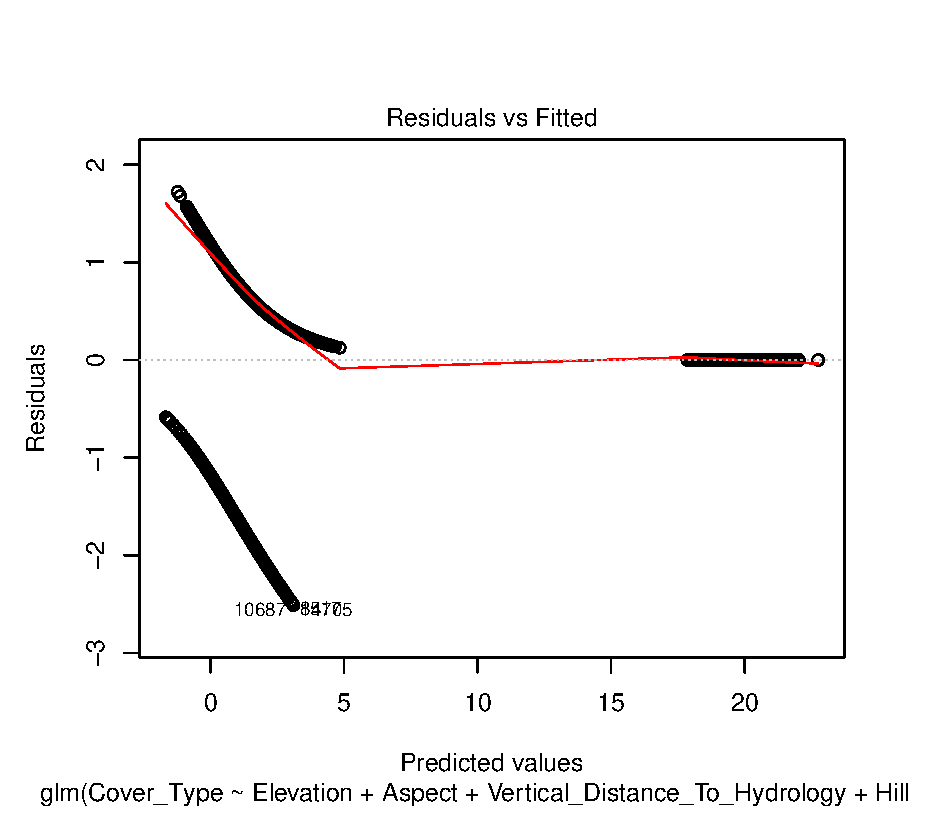
\includegraphics[width=0.9\linewidth]{glm1_1}
\caption{Модель glm1, график Residuals vs Fitted}
\label{fig:glm1_1}
\end{figure}
\begin{figure}[H]
\centering
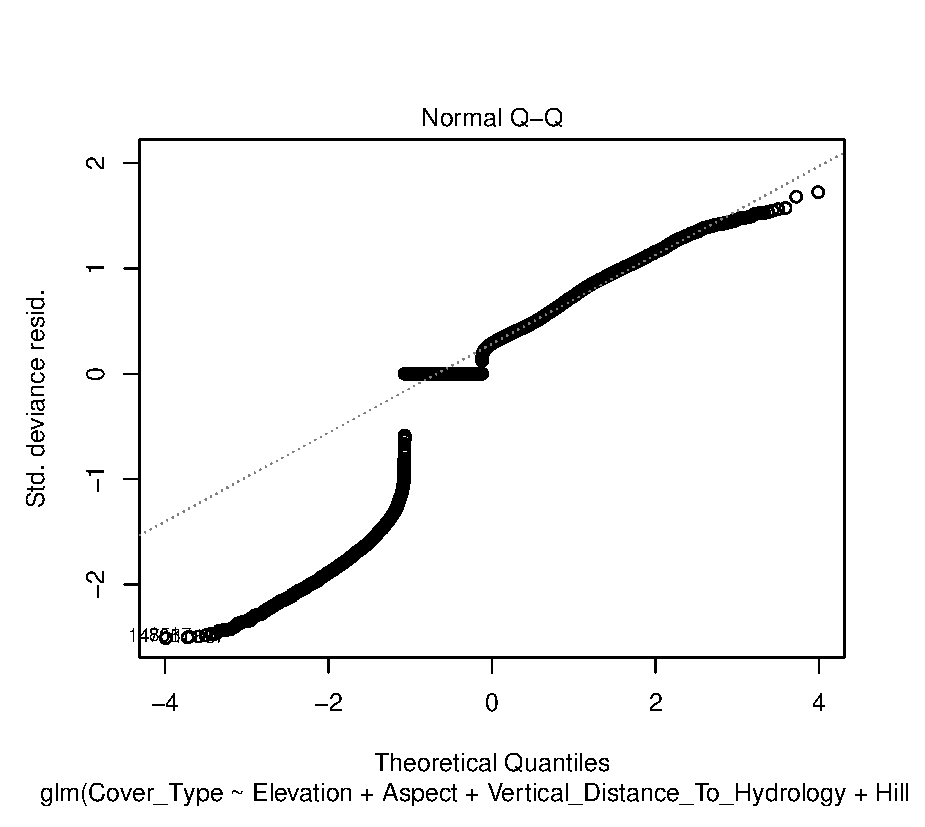
\includegraphics[width=0.9\linewidth]{glm1_2}
\caption{Модель glm1, график Normal Q--Q}
\label{fig:glm1_2}
\end{figure}
\begin{figure}[H]
\centering
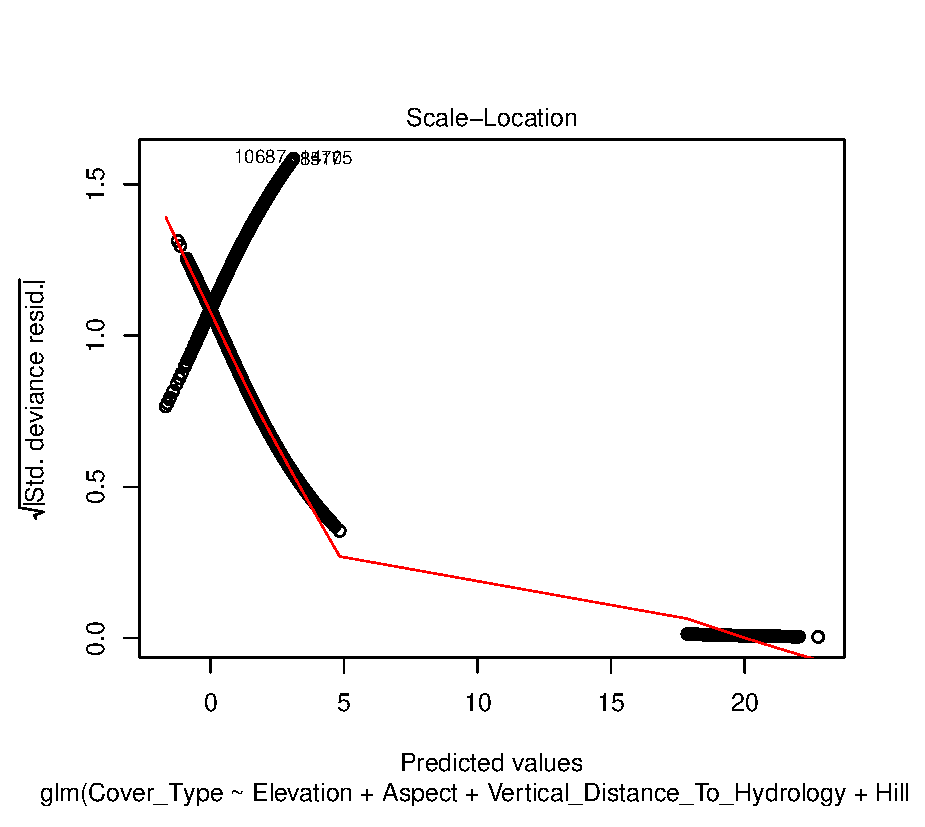
\includegraphics[width=0.9\linewidth]{glm1_3}
\caption{Модель glm1, график Scale--Location}
\label{fig:glm1_3}
\end{figure}
\begin{figure}[H]
\centering
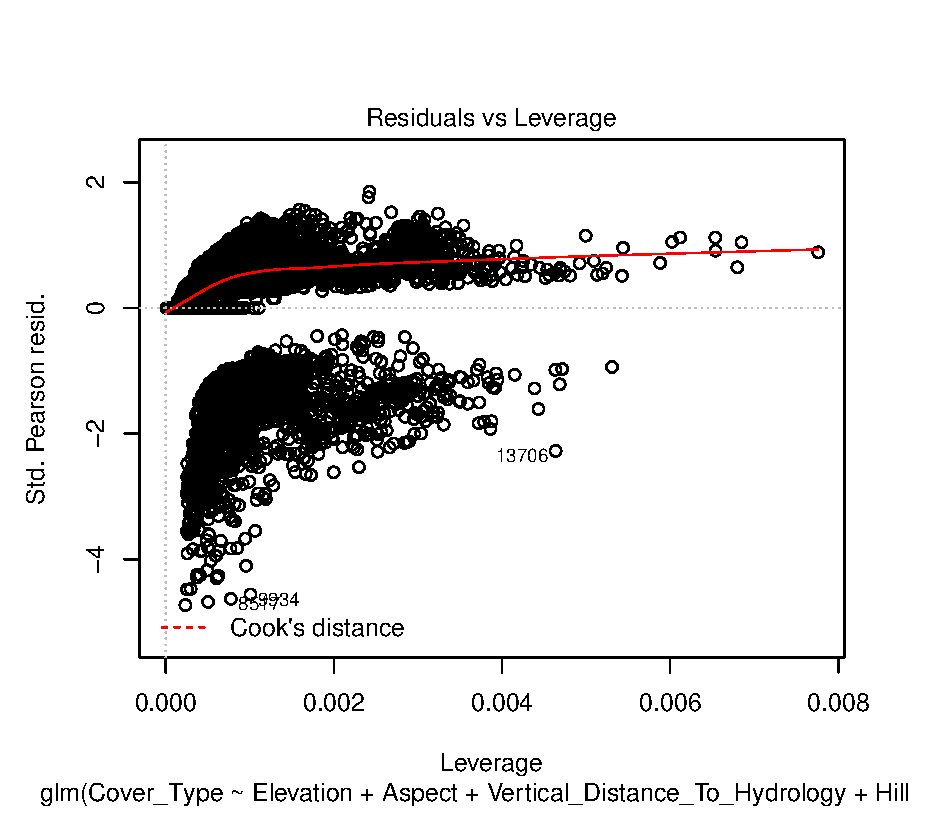
\includegraphics[width=0.9\linewidth]{glm1_4}
\caption{Модель glm1, график Residuals vs Leverage}
\label{fig:glm1_4}
\end{figure}
\end{multicols}

Следует заметить, что графики, как правило, предназначены для линейных регрессионных моделей и плохо визуализируют логистические
(см. также здесь:\\ http://stats.stackexchange.com/questions/121490/interpretation-of-plotglm-model).
Поэтому для валидации модели обратимся непосредственно к численным данным (функции \lstinline[language=r]|summary()|)
\begin{lstlisting}
Call:
glm(formula = Cover_Type ~ Elevation + Aspect + Vertical_Distance_To_Hydrology + 
    Hillshade_Noon + Hillshade_3pm + Horizontal_Distance_To_Fire_Points, 
    family = binomial(), data = df)

Deviance Residuals: 
    Min       1Q   Median       3Q      Max  
-2.6456   0.1512   0.2888   0.5179   1.8841  

Coefficients:
                                     Estimate Std. Error z value Pr(>|z|)    
(Intercept)                         1.025e+01  3.747e-01  27.346  < 2e-16 ***
Elevation                          -3.425e-03  8.683e-05 -39.450  < 2e-16 ***
Aspect                              1.345e-03  2.984e-04   4.508 6.53e-06 ***
Vertical_Distance_To_Hydrology      7.529e-03  4.596e-04  16.382  < 2e-16 ***
Hillshade_Noon                      1.216e-02  1.692e-03   7.188 6.59e-13 ***
Hillshade_3pm                      -1.101e-02  1.052e-03 -10.468  < 2e-16 ***
Horizontal_Distance_To_Fire_Points -7.636e-05  2.210e-05  -3.455 0.000551 ***
---
Signif. codes:  0 ‘***’ 0.001 ‘**’ 0.01 ‘*’ 0.05 ‘.’ 0.1 ‘ ’ 1

(Dispersion parameter for binomial family taken to be 1)

    Null deviance: 12401.9  on 15119  degrees of freedom
Residual deviance:  9718.2  on 15113  degrees of freedom
AIC: 9732.2

Number of Fisher Scoring iterations: 6
\end{lstlisting}
Зедсь уже видно, что данная модель не имеет проблем --- все переменные значимы (p-values для них достаточно малы), значение 
Residual Deviance адекватно (значение \lstinline[language=r]|pchisq(9718.2, 15113)| пренебрежимо мало --- $3.19 \times 10^{-280}$).
Кроме того, с потерей всего 6 ($15119-15113$) степеней свободы отклонение существенно (на 21.6\%, с 12401.9 до 9718.2) уменьшилось.
Поэтому мы можем точно сказать. что принимаем данную модель.

Рассмотрим также модель GAM (для нее пришлось исключить еще часть предположительно незначимых переменных, а также ввести гладкость
по переменной Elevation):
\begin{lstlisting}
gam1 = gam(
  Cover_Type ~ s(Elevation) + Aspect + Vertical_Distance_To_Hydrology
  + Hillshade_Noon + Hillshade_3pm,
  data = df,
  family = binomial()
)
summary(gam1)
\end{lstlisting}
\begin{lstlisting}
Family: binomial 
Link function: logit 

Formula:
Cover_Type ~ s(Elevation) + Aspect + Vertical_Distance_To_Hydrology + 
    Hillshade_Noon + Hillshade_3pm

Parametric coefficients:
                                 Estimate Std. Error z value Pr(>|z|)    
(Intercept)                     2.2884017  0.9447636   2.422  0.01543 *  
Aspect                          0.0010084  0.0003434   2.936  0.00332 ** 
Vertical_Distance_To_Hydrology  0.0033026  0.0005172   6.386  1.7e-10 ***
Hillshade_Noon                  0.0200630  0.0020152   9.956  < 2e-16 ***
Hillshade_3pm                  -0.0127927  0.0012434 -10.289  < 2e-16 ***
---
Signif. codes:  0 ‘***’ 0.001 ‘**’ 0.01 ‘*’ 0.05 ‘.’ 0.1 ‘ ’ 1

Approximate significance of smooth terms:
               edf Ref.df Chi.sq p-value    
s(Elevation) 6.376  6.882   1759  <2e-16 ***
---
Signif. codes:  0 ‘***’ 0.001 ‘**’ 0.01 ‘*’ 0.05 ‘.’ 0.1 ‘ ’ 1

R-sq.(adj) =  0.373   Deviance explained = 41.2%
UBRE = -0.51652  Scale est. = 1         n = 15120
\end{lstlisting}
\begin{figure}[H]
\centering
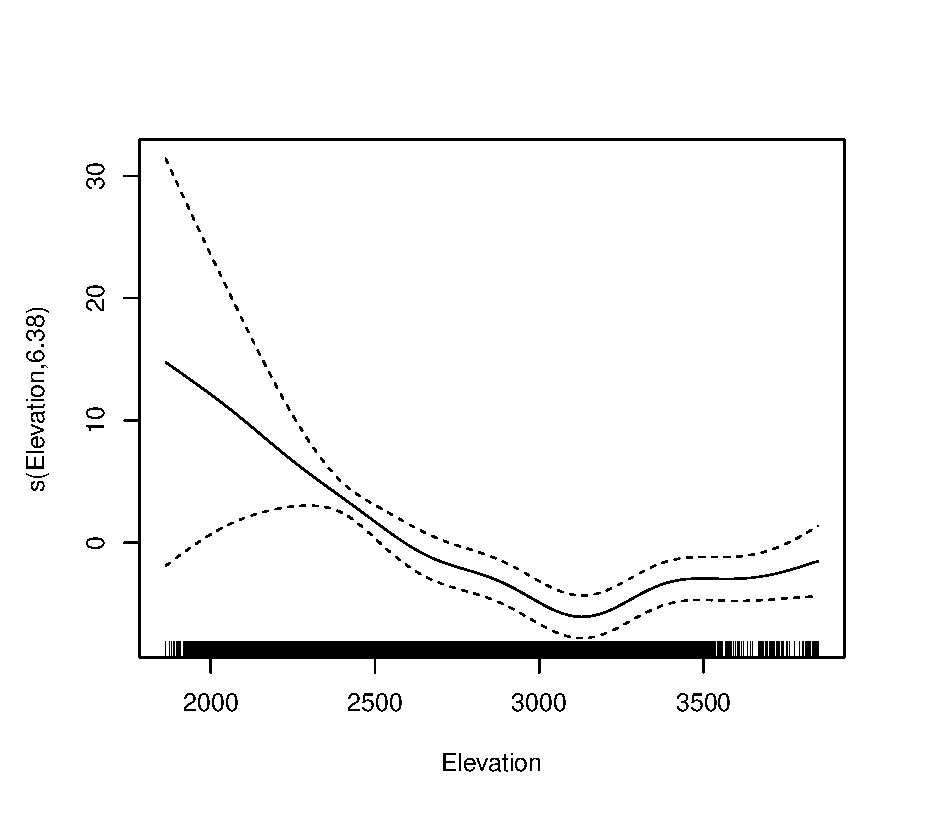
\includegraphics[width=0.9\linewidth]{gam1}
\caption{Модель gam1, график Residuals vs Leverage}
\label{fig:gam1}
\end{figure}
AIC данной модели равен 7310.282.

Как видим, GAM-модель также годится для описания зависимой переменной Cover\_Type.
\end{document}